\chapter {Element Attributes}
\label{c:attrib}
\index{element attribute}

%-----------------------------------------------------------------
\section{Dependent and Independent Attributes} 
\label{s:depend} 
\index{element attribute!dependent and independent}

\index{parameter statement}
\index{dependent attribute}
For convenience, \bmad computes the values of some attributes based
upon the values of other attributes. Some of these dependent variables are
listed in Table~\ref{t:dependent}. Also shown in
Table~\ref{t:dependent} are the independent variables they are
calculated from.  In the table \vn{n_part} and \vn{l_lattice} (lattice
length) are lattice attributes, not element attributes. The first two
are set by the \vn{parameter} statement (See
\sref{s:param}). \vn{l_lattice} is calculated when the lattice is read
in.

\index{bbi_constant}\index{charge}\index{sig_x}\index{sig_y}
\index{e_tot}\index{n_part}\index{e_field}\index{voltage}
\index{hkick}\index{vkick}\index{gap}\index{l}
\index{e_tot}\index{e_loss}\index{delta_e}\index{gradient}
\index{l}\index{rho}\index{angle}\index{l_chord}
\index{g}\index{l}\index{k1}\index{rho}\index{num_steps}\index{ds_step}
\index{b_max}\index{e_tot}\index{beambeam}\index{elseparator}
\index{lcavity}\index{rbend}\index{sbend}\index{wiggler}
\begin{table}[ht]
\centering {
\begin{tabular}{|l|l|l|} \hline
 {\em Element}                & {\em Independent Variables}    & {\em Dependent Variables}          \HH
 All elements                 & \vn{ds_step}                   & \vn{num_steps}                     \HH
 \vn{BeamBeam}                & \vn{charge}, \vn{sig_x}, \vn{sig_y}, \vn{e_tot}, \vn{n_part}
                                                               & \vn{bbi_constant}                  \HH
 \vn{Elseparator}             & \vn{hkick}, \vn{vkick}, \vn{gap}, \vn{l}, \vn{e_tot}      
                                                               & \vn{e_field}, \vn{voltage}         \HH
 \vn{Lcavity}                 & \vn{gradient}, \vn{l}          & \vn{e_loss}, \vn{voltage}          \HH
 \vn{Rbend}, \vn{Sbend}       & \vn{g}, \vn{l}                     
                                                               & \vn{rho}, \vn{angle}, \vn{l_chord} \HH

 \vn{Wiggler} (map type)      & \vn{term(i)}                   & \vn{b_max}, \vn{k1}, \vn{rho}      \HH
 \vn{Wiggler} (periodic type) & \vn{b_max}, \vn{e_tot}         & \vn{k1}, \vn{rho}                  \HH
\end{tabular}
}
\caption[Table of dependent variables.]{Partial listing of dependent variables and 
  the independent variables they are calculated from.}
\label{t:dependent}
\end{table}

\index{lattice!expansion}\index{harmon}\index{delta_e}\index{gradient}
\index{rho}\index{g}\index{angle}\index{rf_frequency}
No attempt should be made to set or vary within a program dependent
attributes. It should be remarked that this is not an iron clad rule.
If a program properly bypasses \bmad's attribute bookkeeping routine
then anything is possible. In a lattice file, before lattice expansion
(\sref{s:expand}), \bmad allows the setting of a select group of
dependent attributes if the appropriate independent attributes are
not set. The list of settable dependent variables is given in
Table~\ref{t:dep.except}.  After reading in the lattice \bmad will set
the appropriate independent variable based upon the value of the
dependent variable. \vn{harmon} is the exception in that it will never
be set by the bookkeeping routine.
\index{lcavity}\index{rbend}
\index{sbend}\index{rfcavity}
\begin{table}[ht]
\centering {
\begin{tabular}{|l|l|l|} \hline
{\em Element}                  & {\em Dependent Variable Set}  &  {\em Independent Variables Not Set} \HH
  \vn{Lcavity}                 & \vn{voltage}       & \vn{gradient}      \HH
  \vn{Rbend}, \vn{Sbend}       & \vn{rho}           & \vn{g}             \HH
  \vn{Rbend}, \vn{Sbend}       & \vn{angle}         & \vn{g}, or \vn{l}  \HH
  \vn{RFcavity}                & \vn{rf_frequency}  & \vn{harmon}        \HH
  \vn{Wiggler} (periodic type) & \vn{n_pole}        & \vn{l_pole}        \HH
\end{tabular}
}
\caption {Dependent variables that can be set in a primary lattice file.}
\label{t:dep.except}
\end{table}

\index{g}\index{g_err}\index{b_field}\index{bs_field}\index{b_field_err}
\index{b1_gradient}\index{b2_gradient}\index{b3_gradient}\index{ks}
\index{k1}\index{k2}\index{k3}
\index{bl_kick}\index{bl_hkick}\index{bl_vkick}
\index{kick}\index{hkick}\index{vkick}
The normal attribute used to vary the strength of, say, a
\vn{quadrupole} is \vn{k1}.  It is sometimes convenient to be able to
vary the magnetic field strength directly instead. To do this \bmad
has a rule that if the appropriate field attribute appears in the
primary lattice file then it becomes an independent variable and the
normalized strength attribute (the strength attribute normalized by
the reference energy) becomes a dependent variable as tabulated in
Table~\ref{t:dep.field}.
\index{sbend}\index{rbend}\index{solenoid}\index{quadrupole}
\index{sol_quad}\index{sextupole}\index{octupole}
\begin{table}[ht]
\centering {
\begin{tabular}{|l|l|l|} \hline
  {\em Element} & {\em Normalized Strength} & {\em Field Attribute} \HH
  \vn{Sbend}, \vn{Rbend}     & \vn{g}      &  \vn{b_field}        \HH
  \vn{Sbend}, \vn{Rbend}     & \vn{g_err}  &  \vn{b_field_err}    \HH
  \vn{Solenoid, Sol_quad}    & \vn{ks}     &  \vn{bs_field}       \HH
  \vn{Quadrupole, Sol_quad, Sbend, Rbend}            
                             & \vn{k1}     &  \vn{b1_gradient}    \HH
  \vn{Sextupole, Sbend, Rbend}             
                             & \vn{k2}     &  \vn{b2_gradient}    \HH
  \vn{Octupole}              & \vn{k3}     &  \vn{b3_gradient}    \HH
  \vn{HKicker}, \vn{VKicker} & \vn{kick}   &  \vn{bl_kick}        \HH
  Most                       & \vn{hkick}  &  \vn{bl_hkick}       \HH
  Most                       & \vn{vkick}  &  \vn{bl_vkick}       \HH
\end{tabular}
}
\caption {Field and Strength Attributes.}
\label{t:dep.field}
\end{table}
Using both field strength and normalized strength as the independent
variable for a given element is not permitted. For example, for a quadrupole the 
normalized strengths \vn{k1}, \vn{hkick}, and \vn{vkick} can be used as the
independent variable or the field strengths \vn{b1_gradient}, \vn{bl_hkick} and
\vn{bl_vkick}. but the mixing of the two is not valid
\begin{example}
  Q1: quadrupole, k1 = 0.6, bl_hkick = 37.5  ! NO. Not VALID.
\end{example}
\index{field_master}
To define an element with the field strength as the independent
attribute without setting the strength just set the strength to zero
or, alternatively, the \vn{field_master} logical can be set. For
example
\begin{example}
  Q1: quadrupole, b1_gradient = 0   ! Field strengths now the independent variables
  Q1: quadrupole, field_master = T  ! Same as above
\end{example}
The same effect can be obtained by setting the field or \vn{field_master} attributes
after the element has been defined.
\begin{example}
  q1: quadrupole        ! Define q1.
  q1[b1_gradient] = 0   ! Field strengths now the independent variables.
  q1[field_master] = T  ! Same as above.
\end{example}

%-----------------------------------------------------------------
\section{Type, Alias and Descrip Attributes}
\label{s:alias}
\index{type|hyperbf}
\index{alias|hyperbf}
\index{descrip|hyperbf}

There are three string labels associated with any element:
\begin{example}
  type    = <String>
  alias   = <String>
  descrip = <String>
\end{example}
\bmad routines do not use these labels except when printing element
information. \vn{type} and \vn{alias} can be up to 40 characters in
length and \vn{descrip} can be up to 200 characters. The attribute
strings can be enclosed in double quotation marks ("). The attribute
strings may contain blanks. If the attribute string does not contain a
blank then the quotation marks may be omitted. In this case the first
comma (,) or the end of the line marks the end of the string. Example:
\begin{example}
  Q00W: Quad, type = "My Type", alias = Who_knows, &
                                  descrip = "Only the shadow knows"
\end{example}

%-----------------------------------------------------------------
\section[Energy and Wavelength Attributes]{Energy and Wavelength Attributes: E_tot, P0C, and ref_wavelength }
\label{s:energy}
\index{parameter statement}\index{e_tot}
\index{e_tot_start}\index{p0c_start}
\index{patch}\index{lcavity}\index{p0c}\index{e_gun}
\index{n_ref_pass}\index{ref_wave_length}
The attributes that define the reference energy and momentum at an element are:
\begin{example}
  e_tot  = <Real>  ! Total energy in eV.
  p0c    = <Real>  ! Momentum in eV.
\end{example}
The energy and momentum are defined at the exit end of the element.
For ultra--relativistic particles, and for photons, these two values
are the same (\sref{s:phase.space}). Except for multipass elements
(\sref{s:multipass}), \vn{e_tot} and \vn{p0c} are dependent attributes
and, except for multipass elements, any setting of \vn{e_tot} and
\vn{p0c} in the lattice input file is an error. The value of
\vn{e_tot} and \vn{p0c} for an element is calculated by \bmad to be
the same as the previous element except for \vn{e_gun}, \vn{lcavity} and
\vn{patch} elements. To set the \vn{e_tot} or \vn{p0c} at the start of
the lattice use the \vn{beginning} or \vn{parameter} statements.
See~\sref{s:param}. Since the energy changes from the start to the end
of an \vn{lcavity} or. \vn{em_field}, an \vn{lcavity} or \vn{em_field} has
the dependent attributes
\index{em_field}\index{lcavity}
\begin{example}
  e_tot_start   and
  p0c_start
\end{example}
which are just the reference energy and momentum at the start of the element.

\index{init_ele}
The \vn{init_ele} element (\sref{s:init.ele}) also has associated
\vn{e_tot_start} and \vn{p0c_start} attributes as well as \vn{e_tot}
and \vn{p0c}. Generally, for an \vn{init_ele}, \vn{p0c_start} and
\vn{p0c} are the same and \vn{e_tot_start} and \vn{e_tot} are the same
and the values for these attributes are set in the lattice file with
the appropriate \vn{parameter} (\sref{s:param}) or \vn{beginning}
(\sref{s:beginning}) statement. The exception occurs when there is an
\vn{e_gun} element in the lattice (\sref{s:e.gun}). In this case, the
\vn{p0c_start} and \vn{e_tot_start} attributes of the \vn{init_ele}
are set to the values as set in the lattice file and \vn{e_tot} is set
to
\begin{example}
  e_tot = e_tot_start + voltage
\end{example}
and \vn{p0c} is calculated from \vn{e_tot} and the mass of the
particle being tracked. For example, if the lattice file contained:
\begin{example}
  beginning[p0c] = 0
  gun: e_gun, voltage = 0.5e6
  injector: line = (gun, ...)
\end{example}
Then the following energy values will be set for the beginning \vn{init_ele} element:
\begin{example}
  p0c_start   = 0
  e_tot_start = mc2
  e_tot       = mc2 + 0.5e6
  p0c         = Sqrt(e_tot - mc2^2)
\end{example}
where \vn{mc2} is the particle rest mass.  The reason for using this
convoluted convention is to allow the setting, in the lattice file, of
a zero reference momentum at the start of the lattice, while
avoiding the calculational problems that would occur if the \vn{e_gun}
element truly had a starting reference momentum of zero.
Specifically, the problem with zero reference momentum is that the
phase space momentum would be infinity as can be seen from \Eqs{ppp}.

For \vn{multipass} elements, the reference energy is set by specifying
one of \vn{e_tot}, \vn{p0c}, or \vn{n_ref_pass} as described in
\sref{s:multipass}.

For photons, the reference wavelength, \vn{ref_wavelength} is also a
dependent attribute calculated from the reference energy.

%-----------------------------------------------------------------
\section{Offset, Pitch, Tilt, and Roll Attributes}
\label{s:offset}\index{x_offset|hyperbf}
\index{y_offset|hyperbf}\index{s_offset|hyperbf}
\index{x_pitch|hyperbf}\index{y_pitch|hyperbf}
\index{roll|hyperbf}\index{tilt|hyperbf}

There are up to 7 attributes that can offset a physical element
from the reference orbit. They are
\begin{example}
  x_offset = <Real>
  y_offset = <Real>
  s_offset = <Real>
  x_pitch  = <Real>
  y_pitch  = <Real>
  tilt     = <Real>
  roll     = <Real>
\end{example}
\index{patch}
The exception here is the \vn{patch} element which uses these
attributes to modify the reference orbit itself.

\vn{x_offset} translates an element in the local $x$--direction
as shown in \fig{f:pitch}. Similarly, \vn{y_offset} and 
\vn{s_offset} translate an element along the local $y$ and 
$z$--directions respectively. For a bend it is assumed that
the bend angle is small and the rotation of the local reference
axes through the bend is ignored.

The \vn{x_pitch} and \vn{y_pitch} attributes rotate an element such
that the unit $z$-axis vector attached to the element, in terms of the
laboratory coordinate frame, is given by
\begin{example}
  \((z\sb{x}, z\sb{y}, z\sb{z})\) = \((s\sb{x}, s\sb{y}, \sqrt{1 - s\sb{x}\sp{2} - s\sb{y}\sp{2}})\)
  Where: \(s\sb{x}\) = sin(x_pitch), and  \(s\sb{y}\) = sin(y_pitch)
\end{example}
and the rotation axis is perpendicular to the laboratory $z$-axis and
the element $z$-axis. Transformation formulas between labortory and
element reference frames is given in \sref{s:lab.ele.coord}.

If \vn{y_pitch} is zero, The \vn{x_pitch} attribute rotates an element
about the $y$--axis so that the exit face of the element is displaced
in the $+x$--direction as shown in figure~\ref{f:pitch}. Similarly, if
\vn{x_pitch} is zero, the \vn{y_pitch} attribute rotates an element
about the $x$--axis so that the exit face of the element is displaced
in the $+y$--direction. The rotations are about the center of the
element which is in contrast to the \vn{dtheta} and \vn{dphi}
misalignment of \mad which rotate around the entrance point. In terms
of rotation angle
\index{MAD!element rotation origin}
\begin{example}
  x_pitch (Bmad) =  dtheta (MAD)
  y_pitch (Bmad) = -dphi (MAD)
\end{example}

\begin{figure}[t]
  \centering
  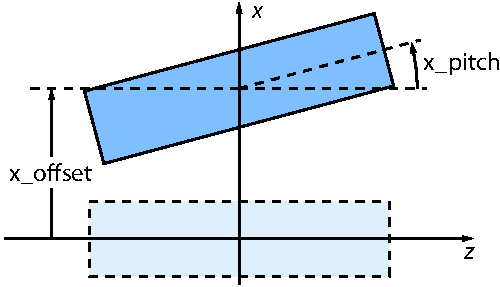
\includegraphics{pitch.pdf}
  \caption{Geometry of Pitch and Offset attributes}
  \label{f:pitch}
\end{figure}

\begin{figure}[t]
  \centering
  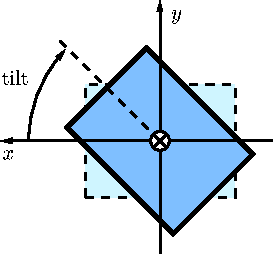
\includegraphics{tilt.pdf}
  \caption{Geometry of a Tilt}
  \label{f:tilt}
\end{figure}

The tilt attribute rotates the element in the $(x, y)$ plane as shown
in figure~\ref{f:tilt}. The rotation axis is the $z$-axis at the
entrance face. The reference orbit is also rotated for any element
who's exit coordinates are not colinear with the entrance
coordinates. For example, a \vn{bend} or \vn{mirror} with a tilt of
$\pi/2$ will bend a beam vertically upward. The \vn{hkick} and
\vn{vkick} attributes are not affected by \vn{tilt} except for
\vn{kicker} and \vn{elseparator} elements. Like MAD, \bmad allows the
use of the \vn{tilt} attribute without a value to designate a skew
element. For example
\begin{example}
  q1: quad, l = 0.6, x_offset = 0.03, y_pitch = 0.001, tilt
\end{example}
\index{rbend!tilt default}\index{sbend!tilt default}
\index{sol_quad!tilt default}\index{quadrupole!tilt default}
\index{sextupole!tilt default}\index{octupole!tilt default}
Default tilts can be used for \vn{rbend}, \vn{sbend}, \vn{sol_quad},
\vn{quadrupole}, \vn{sextupole}, and \vn{octupole} elements.
The default tilt is $\pi/(2(n+1))$ where $n$ is the order of the 
element (n = 0 for bends, n = 1 for quadrupoles etc.) 

\index{sbend}\index{rbend}\index{crystal}\index{mirror}\index{multilayer_mirror}
For all elements, except \vn{crystal}, \vn{mirror}, and
\vn{multilayer_mirror} elements, offsets and pitches and are measured
with respect to the local coordinates at the center of the element. To
simplify things, since there is no real ``center'' for \vn{crystal},
\vn{mirror}, and \vn{multilayer_mirror} elements, these elements
measure their offsets and pitches with respect to the entrance
coordinates.  Note that all element define \vn{tilt} with respect to
the entrance coordinates.

The \vn{roll} attribute is only used for bends and rotates the bend,
along an axis that runs through the entrance point and exit point as
shown in figure~\ref{f:roll}. A \vn{roll}, unlike a \vn{tilt}, does not affect the
reference orbit. The major effect of a \vn{roll} is to give a vertical
kick to the beam. For a bend with positive bend angle, a positive
\vn{roll} will move the outside portion ($+x$ side) of the bend upward
and the inside portion (-$x$ side) downward. Much like car racetracks
which are typically slanted towards the inside of a turn.

\begin{figure}[ht]
  \centering
  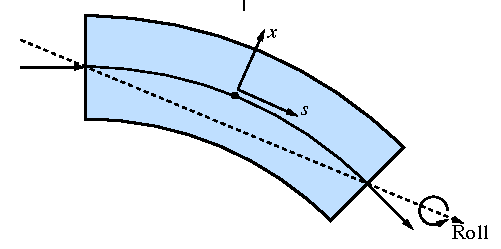
\includegraphics{roll.pdf}
  \caption[Geometry of a Bend]{
Geometry of a Bend. A roll is a rotation around the axis passing
through the entrance and exit points. Like most other elements,
offsets and pitches are calculated with respect to the coordinates at
the center of the bend. Shown here is the geometry for a bend with
\vn{tilt} = 0. That is, the bend is in the $x-s$ plane.}
  \label{f:roll}
\end{figure}

\index{x_offset_tot|hyperbf}\index{y_offset_tot|hyperbf}\index{s_offset_tot|hyperbf}
\index{x_pitch_tot|hyperbf}\index{y_pitch_tot|hyperbf}
\index{tilt_tot|hyperbf}
If an element is supported by a \vn{girder} element (\sref{s:girder}),
the offsets, pitches and tilt of the element are with respect to the
orientation of the \vn{girder}. The computed offsets, pitches and tilt with
respect to the local reference coordinates are stored in the dependent attributes
\begin{example}
  x_offset_tot
  y_offset_tot
  s_offset_tot
  x_pitch_tot
  y_pitch_tot
  tilt_tot
\end{example}
If an element is not supported by a \vn{girder}, \vn{x_offset_tot}
will have the same value as \vn{x_offset} etc.

%-----------------------------------------------------------------
\section{Hkick, Vkick, and Kick Attributes}
\label{s:kick}
\index{hkick|hyperbf}\index{bl_hkick|hyperbf}
\index{vkick|hyperbf}\index{bl_vkick|hyperbf}
\index{kick|hyperbf}\index{bl_kick|hyperbf}


\index{hkicker}
\index{vkicker}
\index{elseparator}
\index{kicker}
The kick attributes that an element may have are:
\begin{example}
  kick,  bl_kick  = <Real>  ! Used only with a Hkicker or Vkicker
  hkick, bl_hkick = <Real>
  vkick, bl_vkick = <Real>
\end{example}
\vn{kick}, \vn{hkick}, and \vn{vkick} attributes are the integrated
kick of an element in radians. \vn{kick} is only used for \vn{hkicker}
and \vn{vkicker} elements. All other elements that can kick use
\vn{hkick} and \vn{vkick}. The \vn{tilt} attribute will only rotate a
kick for \vn{hkicker}, \vn{vkicker}, \vn{elseparator} and \vn{kicker}
elements. This rule was implemented so that, for example, the
\vn{hkick} attribute for a skew quadrupole would represent a
horizontal steering. The \vn{bl_kick}, \vn{bl_hkick}, and
\vn{bl_vkick} attributes are the integrated field kick in
\vn{meters-Tesla}. Normally these are dependent attributes except if
they appear in the lattice file (\sref{s:depend}).

%-----------------------------------------------------------------
\section{Aperture and Limit Attributes}
\label{s:limit}
\index{aperture|hyperbf}
\index{limit|hyperbf}
\index{aperture_at|hyperbf}

\begin{figure}[ht]
  \centering
  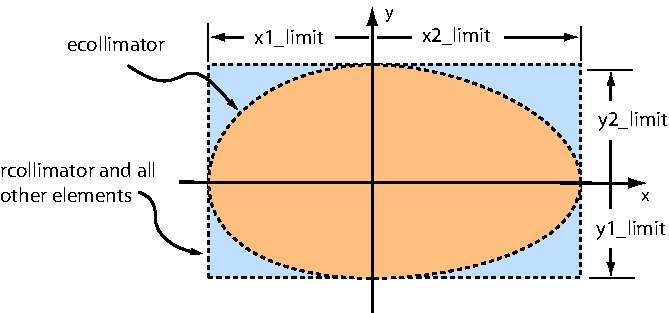
\includegraphics{apertures.pdf}
  \caption[Apertures for ecollimator and rcollimator elements.]
  {Apertures for ecollimator and rcollimator elements. 
  Positive $s$ points up out of the page.}
  \label{f:limit}
\end{figure}

\index{ecollimator}
\index{rcollimator}
\index{x_limit|hyperbf}
\index{y_limit|hyperbf}
\index{x1_limit|hyperbf}
\index{y1_limit|hyperbf}
\index{x2_limit|hyperbf}
\index{y2_limit|hyperbf}
\index{x_offset|hyperbf}
\index{offset_moves_aperture|hyperbf}
\index{aperture_type}
The aperture attributes are:
\begin{example}
  x1_limit      = <Real>      ! Horizontal, negative side, aperture limit
  x2_limit      = <Real>      ! Horizontal, positive side, aperture limit
  y1_limit      = <Real>      ! Vertical, negative side, aperture limit
  y2_limit      = <Real>      ! Vertical, positive side, aperture limit
  x_limit       = <Real>      ! Alternative to specifying x1_limit and x2_limit
  y_limit       = <Real>      ! Alternative to specifying y1_limit and y2_limit
  aperture      = <Real>      ! Alternative to specifying x_limit and y_limit
  aperture_at   = <Switch>    ! What end aperture is at.
  aperture_type = <Switch>    ! What type of aperture it is.
  offset_moves_aperture = <Logical> ! Element offsets affect aperture position
\end{example}
\vn{x1_limit}, \vn{x2_limit}, \vn{y1_limit}, and \vn{y2_limit} specify
the half--width of the aperture of an element as shown in
figure~\ref{f:limit}. A zero \vn{x1_limit}, \vn{x2_limit},
\vn{y1_limit}, or \vn{y2_limit} is interpreted as no aperture in the
appropriate plane.

By default, apertures are assumed to be
rectangular except that an \vn{ecollimator} has a elliptical aperture.
This can be changed by setting the \vn{aperture_type} attribute. The possible 
values of this attribute are:
\begin{example}
  rectangular
  elliptical
  custom
\end{example}
The \vn{custom} setting is used in the case where programs have been
compiled with custom, non-Bmad, code to handle the aperture calculation.

To avoid numerical overflow and other errors in tracking, a particle
will be considered to have hit an aperture in an element, even if
there are no apertures set for that element, if its orbit exceeds 1000
meters. Additionally, there are other situations where a particle will
be considered lost. For example, if a particle's trajectory does
not intersect the output face in a bend.

For convenience, \vn{x_limit} can be used to set \vn{x1_limit} and
\vn{x2_limit} to a common value. Similarly, \vn{y_limit} can be used
to set \vn{y1_limit} and \vn{y2_limit}.  The \vn{aperture} attribute
can be use to set all four \vn{x1_limit}, \vn{x2_limit}, \vn{y1_limit}
and \vn{y2_limit} to a common value. Internally, the \bmad code does {\em not}
store \vn{x_limit}, \vn{y_limit}, or \vn{aperture}. This means that
using \vn{x_limit}, \vn{y_limit} or aperture in arithmetic expressions is
an error:
\begin{example}
  q2: quad, aperture = q1[aperture]   ! THIS IS AN ERROR!
  q2: quad, aperture = q1[x1_limit]   ! Correct
\end{example}

\index{tilt}
\index{x_offset}
\index{y_offset}
\index{x_pitch}
\index{y_pitch}
\index{rcollimator}\index{ecollimator}
\index{multilayer_mirror}\index{mirror}\index{crystal}
Normally, whether a particle hits an aperture or not is evaluated
independent of any element offsets (\sref{s:offset}). This is
equivalent to the situation where a beam pipe containing an aperture
is independent of the placement of the physical element the beam pipe
passes through. That is, the beam pipe does not ``touch'' the physical
element. This can be changed by setting the \vn{offset_moves_aperture}
attribute to \vn{True}. In this case any offsets or pitches will be
considered to have shifted the aperture boundary. The exceptions here
is that the default for \vn{rcollimator}, \vn{ecollimator},
\vn{multilayer_mirror}, \vn{mirror}, and \vn{crystal} elements is for
\vn{offset_moves_aperture} to be \vn{True}.

Even with \vn{offset_moves_aperture} set to \vn{True}, \vn{tilt}s will
not affect the aperture calculation. This is done, for example, so
that the tilt of a skew quadrupole does not affect the aperture. The
exception here is that tilting an \vn{rcollimator} or \vn{ecollimator}
element will tilt the aperture. Additionally, when the aperture is at
the \vn{surface} (see below), any \vn{tilt} will be used in the
calculation.

\index{both_ends|hyperbf}\index{continuous|hyperbf}
\index{entrance_end|hyperbf}\index{exit_end|hyperbf}
\index{surface|hyperbf}\index{aperture_at}
By default the aperture is evaluated at the exit face only of the
element. This can be changed by setting the \vn{aperture_at} attribute.
Possible settings for \vn{aperture_at} are:
\begin{example}
  entrance_end
  exit_end       ! Default for most elements
  both_ends
  continuous
  surface        ! Default for mirror, multilayer_mirror and crystal
\end{example}
Note that the entrance and exit ends of an element are independent of
which direction particles are tracked through an element. Thus if a
particle is tracked backwards it enters an element at the ``exit end''
and exits at the ``entrance end''. The \vn{continuous} setting
indicates that the aperture is continuous along the length of the
element. This only matters when particle tracking involves stepping
through an element a little bit at a time. For example, as in
Runge-Kutta tracking (\sref{s:tkm}). For tracking where a formula is
used to transform the particle coordinates at the entrance of an
element to the coordinates at the exit end, the aperture is only
checked at the end points so, in this situation, a \vn{continuous}
aperture is equivalent to the \vn{both_ends} setting.

\index{mirror}\index{multilayer_mirror}\index{crystal}
The \vn{surface} setting for \vn{aperture_at} can be only be used for
\vn{mirror}, \vn{multilayer_mirror}, and \vn{crystal} elements.  For
these elements, the \vn{surface} setting is the default.  A setting of
\vn{surface} means that the aperture limits are calculated in the
frame of reference of the surface of the element. To keep things
conceptually simple, if a \vn{surface} aperture is used, the setting
of \vn{offset_moves_aperture} must be set to True (which is the
default for these elements). Non-moving apertures, if desired, can be
setup at the entrance or exit end of the element. Notice that since,
for the \vn{mirror}, \vn{multilayer_mirror}, or \vn{crystal} elements
the offsets and pitches are measured with respect to the entrance-end
coordinates (\sref{s:offset}), it is oftentimes simpler to set up a
separate collimator element positioned at the exit end of the element
than it is to set the exit-end aperture in the element itself. In any
case, extra collimator elements are needed if entrance or exit
collimation is to be used with surface collimation.

Examples:
\begin{example}
  q2: quad, aperture_type = elliptical, aperture_at = continuous
  q1: quad, l = 0.6, x1_limit = 0.045, offset_moves_aperture = T
  q1[y1_limit] = 0.03
  q1[y2_limit] = 0.03
  q1[y_limit] = 0.03  ! equivalent to the proceeding 2 lines.  
  q1[aperture_at] = both_ends
\end{example}

%-----------------------------------------------------------------
\section{Fringe Fields}
\label{s:fringe}
\index{fringe fields}

\index{fringe_type}\index{kill_fringe}
The tracking through the fringe fields of such elements as bends,
quadrupoles, etc is determined by the following element attributes
\begin{example}
  fringe_type    !  
  kill_fringe
\end{example}

The \vn{kill_fringe} may be set to one of
\begin{example}
  no_end               ! Default
  both_ends
  entrance_end
  exit_end
\end{example}
The \vn{kill_fringe} switch is used for vetoing fringe effects at
either of the faces of the element. This is useful in vetoing the
fringe effect in the interior of split elements.

The \vn{fringe_type} may be set to one of the following
\begin{example}
  none              ! Default for non-bend elements.
  basic_bend        ! Default for sbend and rbend elements
  full_bend
  full_straight
\end{example}
The \vn{none} setting ignores any fring fields and is the default for
\vn{quadrupoles}, \vn{sextupoles}, etc. The \vn{basic bend} setting,
which is the default for \vn{rbend} and \vn{sbend} elements, is
essentially the basic vertical focusing effect that is present when
there is a finite \vn{e1} or \vn{e2} face angle. With
\vn{bmad_standard} tracking, \vn{basic_bend} also includes second
order terms.  In some cases, for instance in a chicane,
\vn{basic_bend} is not good enough. With \vn{full_bend} or
\vn{full_straight}, higher order effects are taken into account.  The
difference between \vn{full_bend} and \vn{full_straight} is that with
\vn{full_bend} the fringe field is calculated assuming that there is
translational invariance along the horizontal $x$ axis (as one would have 
in a bend) and for \vn{full_straight} the fring_field i

Eaxmple:
\begin{example}
  b1: rbend, angle = pi/4, g = 0.3, fringe_type = full_bend
\end{example}

\index{ptc_max_fringe_order}
When using PTC tracking (\sref{s:ptc}), the
\vn{parameter[ptc_max_fringe_order]} (\sref{s:param}) determines the maximum
order of the calculated fringe fields.

\index{permfringe}\index{bendfringe}
For programmers who deal with PTC directly: The translation between
\vn{fringe_type} on the \bmad side and \vn{permfringe} and \vn{bendfringe} 
on the PTC side is:
\begin{center}
\begin{tabular}{|l|l|l} \hline
{\em fringe_type} & {\em permfringe} & {\em bendfringe} \\
  none            & False            & False            \\    
  basic_bend      & False            & True             \\    
  full_bend       & True             & True             \\    
  full_straight   & True             & False            \\    
\end{tabular}
\end{center}

%-----------------------------------------------------------------
\section{Surface Curvature for X-Ray elements}
\label{s:s.curve}

Various X-Ray elements, for example a \vn{crystal} (\sref{s:crystal})
element, can have a curved surface. The attributes for specifying the surface curvature are:
\index{d_detec}\index{d_source}\index{g_trans}
\index{c2_curve}\index{c3_curve}\index{c4_curve}
\begin{example}
  c2_curve               = <Real>    ! C2 curvature coefficient.
  c3_curve               = <Real>    ! C3 curvature coefficient.
  c4_curve               = <Real>    ! C4 curvature coefficient.
  d_detec                = <Real>    ! Detector distance.
  d_source               = <Real>    ! Source distance.
  g_trans                = <Real>    ! 1/Radius-of-curvature transverse to the bend plane.
\end{example}

From the input attributes, the following attributes are derived:
\index{c2_curve_tot}\index{c3_curve_tot}\index{c4_curve_tot}
\begin{example}
  c2_curve_tot     ! Total C2 curvature coefficient.
  c3_curve_tot     ! Total C3 curvature coefficient.
  c4_curve_tot     ! Total C4 curvature coefficient.
\end{example}

The curvature of the surface in the plane of the $x$-$z$ plane of the
Element Reference Frame (see \fig{f:crystal}) is determined by
the \vn{d_source}, \vn{d_detec}, \vn{c2_curve}, \vn{c2_curve}, and
\vn{c2_curve} parameters. The curvature is surface is parameterized by
a fourth order polynomial
\Begineq
  -x = c_{2,tot} \, z^2 + c_{3,tot} \, z^3 + c_{4,tot} \, z^4
\Endeq
The coefficients of the polynomial are determined by
\begin{align}
  c_{2,tot} &= \mbox{c2_curve} + \frac{1}{2 \, R_c} \CRNO
  c_{3,tot} &= \mbox{c3_curve} \\
  c_{4,tot} &= \mbox{c4_curve} + \frac{1}{4 \, R_c^3} \CRNO
\end{align}
where 
\Begineq
  \frac{2}{R_c} = \frac{\theta_{g,in}}{d_s} + 
                  \frac{\theta_{g,out}}{d_d}
\Endeq
and
\begin{align}
  d_s &= \begin{cases} 
    \infty & \mbox{d_source} = 0 \\
    \mbox{d_source} & \mbox{otherwise}
  \end{cases} \CRNO
  d_d &= \begin{cases} 
    \infty & \mbox{d_detec} = 0 \\
    \mbox{d_detec} & \mbox{otherwise}
  \end{cases}
\end{align}
\vn{d_source} and \vn{d_detec} can be thought of as distances from the
element to the photon source and detector of photons.  With the above
definitions, and with \vn{c2_curve}, \vn{c3_curve}, and \vn{c4_curve}
equal to zero, photons from the source will be focused on the
detector.

The \vn{g_graze} parameter is equal to 1/\vn{R_graze} where
\vn{R_graze} is the radius of curvature of the element surface in the
bend plane as shown in \fig{f:mirror}. A positive \vn{g_graze}
indicates that the element is concave from the point of view of the
photons. Similarly, the \vn{g_trans} parameter is equal to
1/\vn{R_trans} where \vn{R_trans} is the radius of curvature of the
element surface in the plane transverse to the bend plane. Again, a
positive \vn{g_trans} indicates that the element is concave from the
point of view of the photons.

%-----------------------------------------------------------------

\begin{figure}[tb]
  \centering
  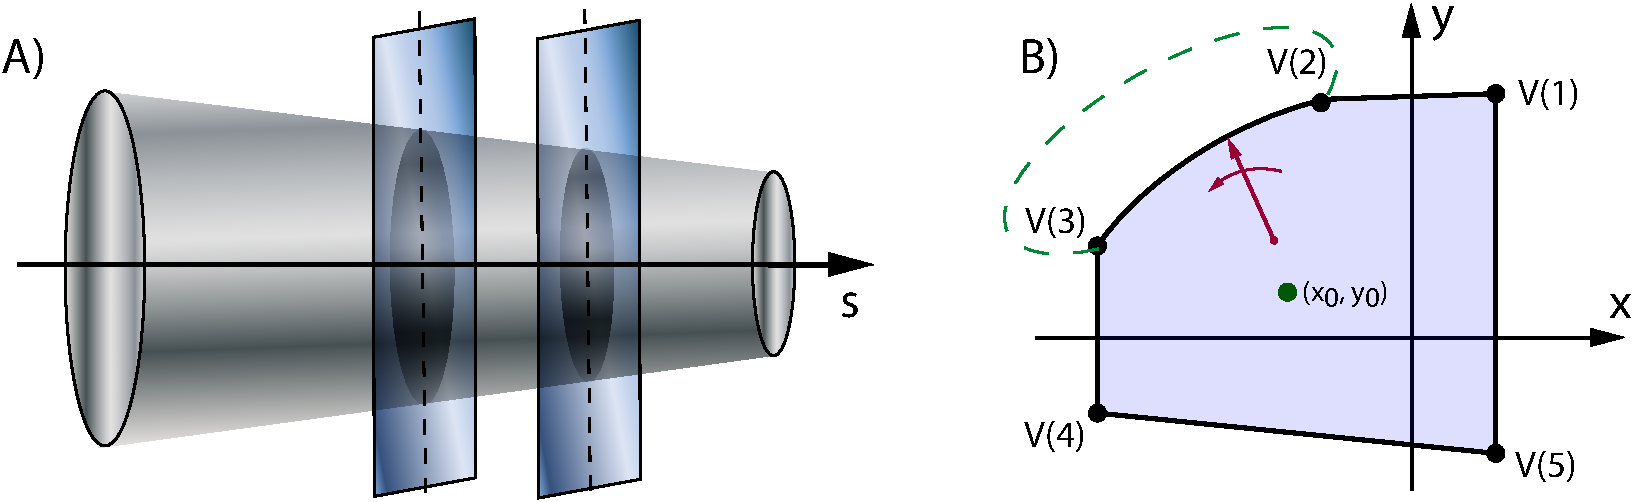
\includegraphics[width=6in]{chamber-wall.pdf}
  \caption[cross-sectional slices of a capillary.]
{A) The inside wall of a capillary or the vacuum chamber wall of a
non-capillary element is defined by a number of cross-sectional
slices.  B) Each cross-section is made up of a number of vertices. The
segments between the vertices can be either a line segment, the arc of
a circle, or a section of an ellipse. The red line segment with one
end at the center of the arc and the other end traversing the arc
from, in this case $V(2)$ to $V(3)$, rotates in counter clockwise
manner. There are two solutions for constructing an arc between two
vertices. The solution with the center point furthest from the origin,
the dashed line between $V(2)$ and $V(3)$ in the figure, is used if
the radius (or radii for an ellipse section) is negative.}
  \label{f:chamber.wall}
\end{figure}

%-----------------------------------------------------------------
\section{Chamber and Capillary Wall}
\label{s:wall}

The vacuum chamber wall shape may be defined for an element using the
\vn{wall} attribute as detailed below. For X-ray capillary elements
(\sref{s:capillary}), this construct is used to define the inside wall
of the capillary.

NOTE: This construct is currently under development. Unless a program
is specifically enabled, the presence of a chamber wall for a
non-capillary element will not affect particle tracking.

The wall is defined by a number of cross-sectional slices as shown in
\fig{f:chamber.wall}A. Each cross-section is defined by a number of
vertices. The arc between each vertex may be either a straight line,
an arc of a circle, or a section of an ellipse. For a capillary it is
mandatory that a cross-section be convex. That is, given any two
points within the cross-section, all points on the line segment
connecting them must be within the cross-section.

\index{wall}\vn{section}\index{s (capillary attribute)}\index{v (capillary attribute)}
\index{dr_ds1}\index{dr_ds1}\index{n_slice_spline}
The \vn{wall} structure defines the capillary wall. The
syntax of the wall structure is:
\begin{example}
  wall = \{
    priority= <rank>,
    section = \{ 
      s = <longitudinal_position>, 
      dr_ds = <value>,
      v(1) = \{<x>, <y>, <radius_x>, <radius_y>, <tilt>\}, 
      v(2) = \{ ... \},
      ...\},
    section = \{
      s = <longitudinal_position>, 
      v(1) = \{... \},
      ... \},
    ... \}
\end{example}
Note: Specifying \vn{priority}, \vn{s_spline} or
\vn{n_cut_spline} is optional. Example:
\begin{example}
  this_cap: capillary, 
    wall = \{   
      priority = primary,
      section = \{ ! cross-section with top/bottom symmetry
        s = 0, v(1) =  \{0.02, 0.00\}, 
        v(2) = \{0.00, 0.02, 0.02\}, v(3) = \{-0.01, 0.01\} \}, 
      section = \{  ! Cross-section that is a tilted ellipse.
        s = 0.34, 
        v(1) = \{0.003, -0.001, 0.015, 0.008, 0.2*pi\} \} \}
\end{example}
In this example an element called \vn{this_cap} is a \vn{capillay}
whose wall is defined by two cross-sections.

The wall structure begins with ``\vn{wall = \{}'' and ends with a
``\vn{\}}''. In between are a number of individual cross-section
structures. Each individual cross-section begins with ``\vn{section =
\{}'' and ends with a ``\vn{\}}''. The \vn{s} parameter of a
cross-section gives the longitudinal position of the cross-section.
For a capillary, \vn{s} must be zero for the first cross-section and
the length of the capillary is given by the value of \vn{s} of the
last cross-section.

The \vn{v(<j>)} within a cross-section define the vertices
for each cross-section. Each \vn{v(<j>)} in turn has five
parameters. It is mandatory to specify the first two parameters
\vn{<x>} and \vn{<y>}. Specifying the rest, \vn{<radius_x>},
\vn{<radius_y>}, and \vn{<tilt>}, is optional. The default values, if
not specified, is zero. The point (\vn{<x>}, \vn{<y>}) defines the
position of the vertex. The parameters \vn{<radius_x>},
\vn{<radius_y>}, and \vn{<tilt>} define the shape of the segment of
the cross-section between the given vertex and the preceding one.
\begin{example}
  <radius_x>  = 0, <radius_y>  = 0   --> Straight line segment.
  <radius_x> != 0, <radius_y>  = 0   --> Circular arc with radius = radius_x
  <radius_x>  = 0, <radius_y> != 0   --> Illegal!
  <radius_x> != 0, <radius_y> != 0   --> Ellipse section.
\end{example}
When an ellipse is specified, \vn{<radius_x>}, and \vn{<radius_y>} are
the half width and half height of the semi-major axes and the
\vn{<tilt>} parameter gives the tilt of the ellipse. \vn{<radius_x>}
and \vn{<radius_y>} must not be negative.

In the example above, for the first cross-section, \vn{v(2)}
specifies a non-zero \vn{<radius_x>} and, by default, \vn{<radius_y>}
is zero. Thus the segment of the cross-section between \vn{v(1)} and
\vn{v(2)} is circular in nature with a radius of 0.02. Since \vn{v(3)}
does not specify \vn{<radius_x>} nor \vn{<radius_y>}, the
cross-section between \vn{v(2)} and \vn{v(3)} is a straight line
segment.

The vertex points must be arranged in a ``counter clockwise manner''. 
For vertices \vn{<v(i)>} and \vn{<v(i+1)>} connected by a line segment
this translates to
\Begineq
  0 < \theta_{i+1} - \theta_{i} \pmod{2\pi} < \pi
\Endeq
where $(r_n, \theta_n)$ are the polar coordinates of the $n^{th}$
vertex. For vertices connected by an arc, ``counter clockwise manner''
means that the line segment with one end at the center of the arc and
the other end traversing the arc from \vn{<v(i)>} to \vn{<v(i+1)>}
rotates in counter clockwise as shown in
\fig{f:chamber.wall}B. In general, there are two solutions for
constructing such an arc. For positive radii, the solution chosen is
the one whose center is closest to the origin.  

A restriction on cross-sections is that the origin $(0,0)$ must be in the
interior of any cross-section and that for any cross-section a line
drawn from the origin at any given angle $\theta$ will intersect the
cross-section at exactly one point as shown in
\fig{f:chamber.wall}B. This is an important point in the
construction of the wall between cross-sections as explained
below.

The last vertex specified, call it \vn{<v(n)>}, should not have the
same \vn{<x>}, \vn{<y>} values as the first vertex \vn{<v(1)>}. That
is, there will be a segment of the cross-section connecting
\vn{<v(n)>} to \vn{<v(1)>}. The geometry of this segment is determined
by the parameters of \vn{<v(1)>}.

If there is mirror symmetry about the $x$ or $y$ axis for a
cross-section, the ``mirrored'' vertices, on the ``negative'' side of
the mirror plane, do not have to be specified. Thus if all the vertex
points of a cross-section are in the first quadrant, that is, all
\vn{<x>} and \vn{<y>} are zero or positive, mirror symmetry about both the
$x$ and $y$ axes is assumed. If all the \vn{<y>} values are zero or
positive and some \vn{<x>} values are positive and some are negative,
mirror symmetry about the $x$ axis is assumed. Finally, if all the
\vn{<x>} values are zero or positive but some \vn{<y>} values are
positive and some are negative, symmetry about the $y$ axis is
assumed. For example, for the first in the above example, since
all the \vn{<y>} values are non-negative and there are positive and
negative \vn{<x>} values, symmetry about the $x$ axis is assumed.

The one exception to the above rule that (\vn{<x>}, \vn{<y>}) is the
vertex center is when a single vertex \vn{v(1)} is specified for a
cross-section with a non-zero \vn{<radius_x>}. In this case,
(\vn{<x>}, \vn{<y>}) are taken to be the center of the circle or
ellipse. In the example above, the second cross-section is a
tilted ellipse with center at $(0.003, -0.001)$. If a cross-section
has a single vertex and \vn{<radius_x>} is
not specified, the cross-section is a rectangle. For example
\begin{example}
    section = \{ s = 0.34, v(1) = \{0.03, 0.01\} \}
\end{example}

\begin{figure}[tb]
  \centering
  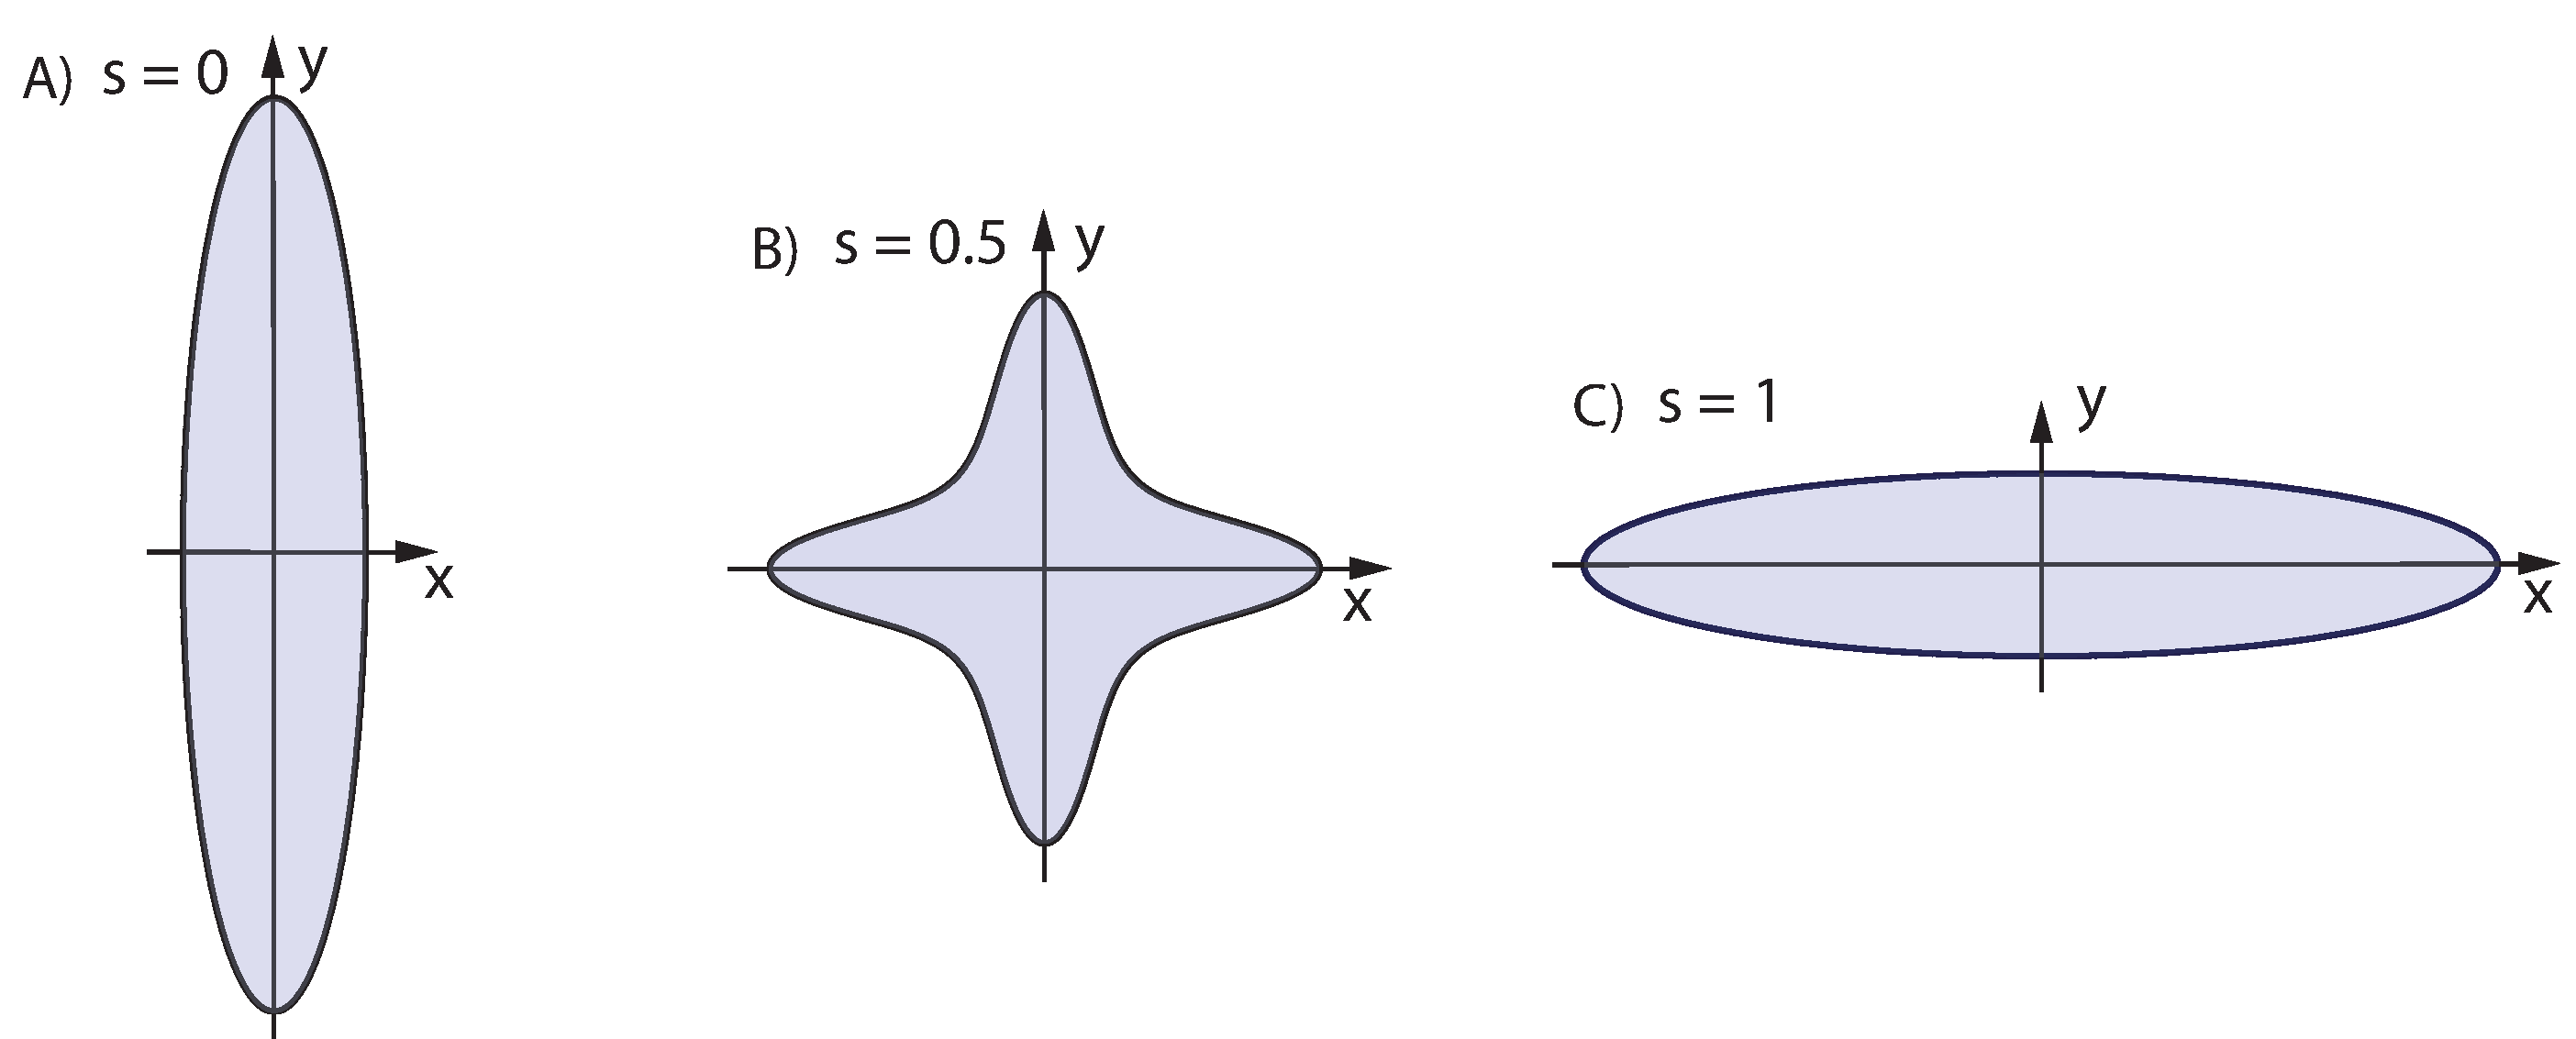
\includegraphics[width=4in]{concave-capillary.pdf}
  \caption[Convex cross-sections do not guarantee a convex volume.]
{Example where convex cross-sections do not produce a convex volume.
Cross-sections (A) and (C) are ellipses with a 5 to 1 aspect ratio.
Half way in between, linear interpolation produces a convex cross-section
as shown in (B).} 
  \label{f:concave.capillary}
\end{figure}

Between cross-sections, the wall is defined by interpolation. Let
$r_{c1}(\theta)$ be the radius of the wall as a function of $\theta$
for a given cross-section defined at $s = s_1$. Let $r_{c2}(\theta)$
be the radius function at the next defined cross-section at $s =
s_2$. The wall $r_c(\theta, s)$ at any point $s$ between $s_1$ and
$s_2$ is defined by the equation
\Begineq
  r_c(\theta, s) p_1(\stilde) \, r_{c1}(\theta) + p_2(\stilde) \, r_{c2}(\theta)
\Endeq
where 
\Begineq
  \stilde \equiv \frac{s - s_1}{s_2 - s_1}
\Endeq
and $p_1$ and $p_2$ are cubic polynomials parameterized by
\begin{align}
  p_1 &= 1 - \stilde + a_1 \, \stilde + a_2 \, \stilde^2 + a_3 \, \stilde^3 \CRNO
  p_2 &= \stilde + b_1 \, \stilde + b_2 \, \stilde^2 + b_3 \, \stilde^3 
\end{align}
If $a_i = b_i = 0$ for all $i = 1, 2, 3$, the interpolation is linear
and this is the default if the parameters \vn{dr_ds1} and \vn{dr_ds2}
are not given in the wall definition. These parameters are the
slopes of the wall with respect to $s$ at the end points
\begin{equation}
  \mbox{dr_ds1} \equiv \left. \frac{d\overline{r}}{ds} \right|_{s = s_1} \comma \qquad
  \mbox{dr_ds2} \equiv \left. \frac{d\overline{r}}{ds} \right|_{s = s_2} 
\end{equation}
where $\overline{r}$ is the average $r$ averaged over all
$\theta$. When \vn{dr_ds1} and \vn{dr_ds2} are specified, the $a_i$
and $b_i$ are calculated so that the slopes of the wall match 
the values of \vn{dr_ds1} and \vn{dr_ds2} along with the constraints.
\begin{align}
  p_1(0) &= 1 \comma \qquad p_1(1) = 0 \CRNO
  p_2(0) &= 0 \comma \qquad p_2(1) = 1 \\
  M &\equiv a_1^2 + a_2^2 + a_3^2 + b_1^2 + b_2^2 + b_3^2 \mbox{ is a minimum}
  \nonumber
\end{align}
The last constraint ensures a ``smooth'' transition between the two cross-sections.

For a capillary, in order for \bmad to quickly track photons,
\bmad assumes that the volume between the cross-sections is
convex. The volume will be convex if each cross-section $r_c(\theta,
s)$ at any given $s$ is convex. Note that it is {\em not} sufficient
for $r_c(\theta, s)$ to be convex at the specified cross-sections as
shown in \fig{f:concave.capillary}. Also note that it is perfectly
fine for the total capillary volume to not be convex.

To refer to a cross-section parameters after an element has been
defined, the following syntax is used:
\begin{example}
  ele_name[wall.section(n).v(j).x]   ! x value of j^th vertex of n^th cross-section
\end{example}

As an alternative, if an element defines an aperture (\sref{s:limit}
with \vn{aperture_at} set to \vn{continuous}, and the element does
{\it not} have a \vn{wall} structure defined for it, then the aperture
defines the wall. By definition, such a wall has a constant cross-section.

When superimposing elements (\sref{s:super}), there is the problem of
how to superimpose walls. If only one of the superimposed elements has
a wall then this wall is used. If more than one superimposed elements
has a wall then the wall with the highest \vn{priority} is used. The
\vn{priority} switch in the wall structure can be set to one of
\begin{example}
  ignore
  secondary  [default]
  primary
\end{example}
a wall with \vn{priority} set to \vn{primary} takes precidence over a
\vn{priority} of \vn{secondary}. A wall with \vn{priority} set to
\vn{ignore} is always ignored even when there is no superposition. It
is an error if there are multiple walls with the highest priority are
superimposed. For example, two elements with walls whose \vn{priority}
is set to \vn{secondary} cannot be superimposed on top of one another.

%-----------------------------------------------------------------
\section{Length Attributes}
\label{s:l}

\index{length of elements}
\index{l|hyperbf}
\index{l_chord|hyperbf}
\index{rbend}
\index{sbend}
The length attributes are
\begin{example}
  l       = <Real>  ! 
  l_chord = <Real>  ! Chord length of a bend. Dependent attribute.
\end{example}
The length \vn{l} is the path length of the reference particle. The
one exception is for an \vn{rbend}, the length \vn{l} set in the
lattice file is the chord length (\sref{s:bend}). internally, \bmad
converts all \vn{rbend}s to \vn{sbend}s and stores the chord length
under the \vn{l_chord} attribute.

\index{wiggler}
Note that for \vn{wiggler}s,
the length \vn{l} is not the same as the path length for a particle
with the reference energy starting on the reference orbit.

%-----------------------------------------------------------------
\section{Is_on Attribute}
\label{s:is.on}
\index{is_on|hyperbf}

The \vn{is_on} attribute
\begin{example}
  is_on = <Logical>
\end{example}
is used to turn an element off. Turning
an element off essentially converts it into a drift.
Example
\begin{example}
  q1: quad, l = 0.6, k1 = 0.95
  q1[is_on] = False
\end{example}

\index{aperture}
\index{reference orbit}
\index{reference energy}
\vn{is_on} does not affect any apertures that are set. Additionally,
\vn{is_on} does not affect the reference orbit. Therefore, turning 
off an \vn{lcavity} will not affect the reference energy.

%-----------------------------------------------------------------
\section{Multipole Attributes: An, Bn, KnL, Tn}
\label{s:multip}

\index{multipole!an, bn|hyperbf} 
\index{multipole!knl, tn|hyperbf} 
\index{ab_multipole}
\index{multipole}
\index{radius}
A \vn{multipole} (\sref{s:mult}) element specifies its multipole
components using an Amplitude (\vn{KnL}) and a tilt (\vn{Tn})
\begin{example}
  KnL = <Real>
  Tn  = <Real>  ! Default is $pi$/(2n + 2)
\end{example}
\vn{ab_Multipole} (\sref{s:ab.m}) and all other elements that
have multipole attributes specify the multipoles using normal
(\vn{Bn}) and skew (\vn{An}) components 
\begin{example}
  An = <Real>
  Bn = <Real>
\end{example}
Here \vn{n} ranges from 0
(dipole component) through 20. Example:
\begin{example}
  q1: ab_multipole, b0 = 0.12, a20 = 1e7
\end{example}

Multipole formulas for are given in \sref{s:fields}.  Note that for
\vn{multipole} and \vn{ab_multipole} (but not any other element) a
non-zero dipole component will affect the reference orbit (just like a
normal dipole will).

The \vn{Tn} tilt component without a value takes a default of $pi$/(2n
+ 2) which makes the component \vn{skew}.  Example:
\begin{example}
  m: multipole, k1l = 0.45, t1  ! Skew quadrupole
\end{example}

For everything other than a \vn{multipole} and \vn{ab_multipole}, the
multipole strength is scaled by a factor $F \, r_0^{n_\text{ref}} /
r_0^n$ (cf.~\Eq{ababf}) where $F$ is the strength of the element (for
example $F$ is $K1 \cdot L$ for a quadrupole), and $r_0$ is the
``measurement radius'' and is set by the \vn{radius} attribute. The
default value of $r_0$, if the \vn{radius} is not given, is 1.0.  This
behavior may be turned off by setting the \vn{scale_multipoles}
attribute.  Example:
\begin{example}
  q1: quadrupole, b0 = 0.12, a20 = 1e7, scale_multipoles = F
\end{example}

%-----------------------------------------------------------------
\section{Electromagnetic Fields}
\label{s:em.fields}

\index{lcavity}\index{rfcavity}\index{em_field}\index{field}
3D Electromagnetic fields can be specified using the \vn{field}
attribute. Fields so specified can be used with, for example,
\vn{runge_kutta} tracking (\sref{s:tkm}), etc. The \vn{field}
attribute can be used with both RF and DC fields however RF fields can
only be associated with \vn{lcavity}, \vn{rfcavity}, and \vn{em_field}
elements.

The syntax for specifying the electromagnetic fields is
\index{m}\index{field}\index{mode}\index{freq}\index{dphi0_ref}
\index{f_damp}\index{field_scale}\index{master_scale}\index{phi0_azimuth}
\index{map}\index{grid}
\begin{example}
  field = \{
    mode = \{
      m             = <Integer>, ! Mode number
      harmonic      = <Integer>, ! Harmonic number 
      dphi0_ref     = <Real>,    ! Phase of oscillations.
      f_damp        = <Real>,    ! Oscillation damping factor. Default = 0.
      field_scale   = <Real>,    ! Scale factor for the E & B fields.
      master_scale  = <Name>,    ! Master scaling parameter for E & B fields.
      phi0_azimuth  = <Real>,    ! Azimuthal orientation.
      map           = <EM_field_map>,        ! EM field map data
      grid          = \{<EM_field_grid>\} \},    ! EM field grid data
    mode = \{...\}\}
\end{example}
The electromagnetic field is specified as a series of \vn{modes}. Each
\vn{mode} has a \vn{harmonic} number which, if non-zero, identifies it
as an RF field. The field associated with a mode can be specified
using a \vn{grid} of data points or by a \vn{map} which specify the
coefficients of an analytical form for the field.

The field is scaled by two values specified by \vn{field_scale} and
\vn{master_scale}. That is
\begin{equation}
  [E, B] (actual) = [E, B] (from map or grid) * field_scale * master_scale_value
\end{equation}
That is, the actual field is the value as determined from the \vn{map}
or \vn{grid} data (see below) scaled by the value of \vn{field_scale}
times the ``master_scale_value''. This master_scale_value is the value
of the element parameter given by \vn{master_scale}. For example, for
a quadrupole element, if \vn{master_scale} is set to "K1" then the
fields are scaled by the quadrupole strength parameter. The purpose of
this \vn{master_scale} is to provide a way to scale the 3D fields with
the element strength parameter (K1 for a quadrupole) and also provide
a way to scale separate \vn{mode}s jointly.

The \vn{map} specification has the form
\begin{example}
  map = \{
    dz        = <Real>,    ! Distance between sampled field points.
    e_coef_re = (<Real>, <Real>, ....),  ! Real part of e.
    e_coef_im = (<Real>, <Real>, ....),  ! Imaginary part of e.
    b_coef_re = (<Real>, <Real>, ....),  ! Real part of b.
    b_coef_im = (<Real>, <Real>, ....),  ! Imaginary part of b.
  \}
\end{example}
For rf fields the basic equations used for the mode decomposition of
the rf fields are given in Section~\sref{s:rf.fields.phys}. 
\vn{e_re} and \vn{e_im} give the real an imaginary part of $e$ and
\vn{b_re} and \vn{b_im} give the real and imaginary part of $b$. All
of these vectors must be present and have the same length. The
exception is with an $m = 0$ mode either the $e$ or $b$ arrays can be
omitted and will default to zero. The number of terms $N$ for the $e$
or $b$ vectors must be a power of $2$ and all modes must have the same
number of terms. The $n$\Th element in the $e$ or $b$ arrays, with $n$
running from 0 to $N-1$, is associated with a wavelength $k_n$
\begin{equation}
  k_n = \begin{cases}
    \frac{2 \, \pi \, n}{N \, dz} & n < \frac{N}{2} \\
    \frac{2 \, \pi \, (n-N)}{N \, dz} & \mbox{otherwise}
  \end{cases}
\end{equation}
This convention follows the convention used by Numerical
Recipes\cite{b:nr}.  

The longitudinal length
of the field is
\begin{equation}
  L_{\mbox{field}} = \frac{N - 1}{dz}
\end{equation}
this may be different from the length \vn{l} specified for the
element. If there is a difference, the field is assumed to be centered
on the element and drifts will be used at the entrance and exit ends
of the element to make up the difference.

Alternatively, a grid of field points may be specified. The general format is:
\begin{example}
  grid = \{ 
    type = <String>,
    r0   = (<Real>, <Real>, <Real>),  ! Grid origin 
    dr   = (<Real>, <Real>, <Real>),  ! Grid spacing
    ele_anchor_pt = <Position>        ! BEGINNING, CENTER, or END
    pt(<Integer>, <Integer>, <Integer>) = ( (<Real>, <Real>), \ldots ),  ! Grid field points
    \ldots \}
\end{example}
Currently the only available value for the grid \vn{type} is 
\begin{example} 
  rotationally_symmetric_rz
\end{example} 
The format for this type of grid is 
\begin{example}
  grid = \{ 
    type = rotationally_symmetric_rz,
    r0   = (<r(0,0)>,  <z(0,0)>),     ! Grid origin 
    dr   = (<delta_r>, <delta_z>),    ! Grid spacing
    pt(i_r, i_z) = ((<Re(E_r)>, <Im(E_r)), (<Re(E_phi)>, <Im(E_phi)>), (<Re(E_z)>, <Im(E_z)>))
    \ldots \}
\end{example}

The field of a given mode oscillates as given by Eq.~\ref{eseei}  
\Begineq
  e^{-i \, 2 \, \pi ( f \, t + \theta_0)}
\Endeq
The phase of the oscillation, $\theta_0$ comes from two
sources: the phase \vn{dphi0_ref} set for the mode and an overall phase
\vn{phi_ref} given by
\begin{example}
 phi_ref = phi0 + dphi0
\end{example}
\index{lcavity!reference phase}\index{rfcavity!reference phase}
Unfortunately, to be consistent with \mad, the definition of
\vn{phi_ref} for an \vn{lcavity} (\sref{s:lcav}) differs in sign to
that for an \vn{rfcavity} (\sref{s:rfcav}). This being the case,
$\theta_0$ is
\Begineq
  \theta_0 = 
  \begin{cases}
    \mbox{dphi0_ref} + \dsfrac{f}{f_0} \, (\mbox{phi_ref} + \mbox{phi0_err}) & 
    \mbox{lcavity element} \\
    \mbox{dphi0_ref} - \dsfrac{f}{f_0} \, \mbox{phi_ref} & 
    \mbox{rfcavity element}
  \end{cases}
\Endeq
where $f$ is the mode frequency and $f_0$ is the frequency of the fundamental.

The phase \vn{dphi0_ref} of the fundamental mode is auto-scaled by Bmad
so that a particle with $z = 0$ will go through the cavity on crest
for a \vn{lcavity} and on the zero-crossing for an
\vn{rfcavity}. Additionally, the field of the fundamental mode is
adjusted by an overall factor so that for an \vn{lcavity} the maximal
acceleration is equal to \vn{gradient * L} and for an \vn{rfcavity}
the maximal acceleration is equal to \vn{e * voltage}.

%-----------------------------------------------------------------
\section{RF Couplers}
\label{s:rf.coupler}

\index{lcavity}\index{rfcavity}
\index{coupler_at}\index{coupler_strength}
\index{coupler_angle}\index{coupler_phase}
For \vn{lcavity} and \vn{rfcavity} elements, the attributes that
characterize the dipole transverse kick due to a coupler port are:
\begin{example}
  coupler_at       = <Switch> ! What end the coupler is at
  coupler_strength = <Real>   ! Normalized strength
  coupler_angle    = <Real>   ! Polarization angle (rad/2\(\pi\))
  coupler_phase    = <Real>   ! Phase angle with respect to the RF (rad/2\(\pi\))
\end{example}
The possible \vn{coupler_at} settings are:
\begin{example}
  entrance_end
  exit_end  ! default
  both_ends
\end{example}
For \vn{coupler_angle} = 0 the transverse kick due to the coupler is
\begin{example}
  dp_x = gradient * coupler_strength * 
                        cos(twopi * (phi_ref + coupler_phase + phi(z))) / (c * P_0) 
  dp_y = 0
\end{example}

Example:
\begin{example}
  rf1: lcav, l = 4.5, gradient = 1.2e6, coupler_at = both_ends, coupler_strength = 0.037
\end{example}

%-----------------------------------------------------------------
\section{RF Wakes}
\label{s:rf.wakes}

Wake fields can be specified for \vn{lcavity} and \vn{rfcavity} elements.
The attributes that characterize the wakes are:
\index{sr_wake_file}\index{lr_wake_file}\index{lr_freq_spread}
\begin{example}
  sr_wake_file     = <String> ! Short range wake field definition file.
  lr_wake_file     = <String> ! Long range wake field definition file.
  lr_freq_spread   = <Real>   ! Frequency spread of the LR wake fields.
\end{example}

The formulas used to compute the wake field are given in
\sref{s:wake.fields}.  The input file name for the short--range
wake fields is specified using the \vn{sr_wake_file} attribute. The
file gives both monopole longitudinal and dipole transverse
wakes. Comment lines may be included by starting a line with an
exclamation mark (!). Blank lines are also ignored.  An example input
file is:
\begin{example}
  !    z           Wz             Wt
  !   [m]       [V/C/m]       [V/C/m^2]
   0.000E+00  1.61125E+15   0.00000E+00     1 
  -1.000E-05  1.44516E+15  -1.30560E+15     2 
  -2.000E-05  1.38148E+15  -2.50665E+15     3 
  .. etc ..
  -1.970E-03  3.49958E+14  -7.95507E+16   198 
  -1.980E-03  3.48606E+14  -7.97253E+16   199  
  -1.990E-03  3.47263E+14  -7.98989E+16   200
     END_SECTION


  ! Pseudo Wake modes:
  !                      Amp       damp          k      phase
  ! Longitudinal:      [V/C/m]     [1/m]      [1/m]     [rad]  
  ! Transverse:      [V/C/m^2]     [1/m]      [1/m]     [rad]  

  &short_range_modes
    longitudinal(1) = 3.23e14     1.23e3     3.62e3     0.123
    longitudinal(2) = 6.95e13     5.02e2     1.90e3    -1.503
    .. etc ..
    transverse(1) =   4.23e14     2.23e3     5.62e3     0.789
    transverse(2) =   8.40e13     5.94e2     1.92e3     1.455
     .. etc ..
    z_max = -1.3e-3
  /
\end{example}
The file is divided into two sections with a line containing the word
\vn{END_SECTION} marking the division between the sections.  Wakes can
be specified via a table of wake versus longitudinal position $z$
and/or using a set of ``pseudo'' modes (\sref{s:wake.fields}). The
first section gives the wake vs $z$ table, and the second section
gives the longitudinal monopole and transverse dipole pseudo modes.
The range of the table is from $0$ to $z_{cut}$ where $z_{cut}$ is the
$z$ value in the last line of the table. If the longitudinal distance
$dz$ between two particles is within the range of the table then the
table will be used to calculate the wake kick for this pair. If $dz$
is larger than $z_{cut}$ the pseudo modes will be used. The pseudo
modes are valid from $z_{cut}$ to \vn{z_max}. 

In the first section with the table of wake vs. $z$, the first column is the
longitudinal distance $z$. $z$ must start at 0 and must increment by the a
constant amount from row to row. $z$ is negative since the wake extends behind
a particle. The second column is the longitudinal wake function in $V/C/m$. The
third column is the transverse wake in $V/C/m^2$. Any additional columns are
ignored.  Wake field formulas are to be found in \sref{s:wake.fields}.  The
wake field file is only used with macroparticle and particle distribution
tracking.  When the short--range wake field file is used with either of these
the \vn{e_loss} attribute is ignored. However, even in this case, a finite
\vn{e_loss} value will affect the reference energy. Since the quantities like
quadrupole k1 strengths and bend strengths are referenced to the reference
energy, The value of \vn{e_loss} will affect the results even with a
short--range wake field file.

The input file name for the long--range wake fields is specified using
the \vn{lr_wake_file} attribute. The file gives the
wake modes by specifying the frequency (in Hz), R/Q (in
$\Omega$/meter$^{2m}$), Q, and m (order number), and optionally the
polarization angle (in radians/2pi) for each cavity mode. The input
uses Fortran90 namelist syntax: The data begins with the string
\vn{\&long_range_modes} and ends with a \vn{/}. Everything outside is
ignored. Each mode is labeled \vn{lr(i)} where \vn{i} is the mode
index. An example input file is:
\begin{example}
              Freq      R/Q      Q    m   Polar   b_sin  b_cos a_sin  a_cos  t_ref 
                      [Ohm/               Angle 
              [Hz]     m^(2m)]           [Rad/2pi]
  &long_range_modes
    lr(1) = 1.650e9    0.76    7.0e4  1    unpol
    lr(2) = 1.699e9   11.21    5.0e4  1    0.15
    lr(3) =    0       0.57    1.1e6  0    unpol
  /
\end{example}
A frequency of zero is used to designate wakes that are part of the
fundamental accelerating mode. \bmad needs to know if a wake is part
of the fundamental mode due to timing issues as discussed in \sref{s:rf.time}.

If the polarization angle is set to ``\vn{unpolarized}''
the mode is taken to be unpolarized.

\vn{lr_freq_spread} is used to randomly spread out the long range mode
frequencies among different cavities. The spread is Gaussian in shape
with an RMS of \vn{lr_freq_spread} * $F$ where $F$ is the frequency of a
mode.  After the long--range modes have been defined they can be
referenced or redefined using the notation
\begin{example}
  lr(n)%freq      ! Frequency
  lr(n)%r_over_q  ! R/Q
  lr(n)%q         ! Q
  lr(n)%angle     ! Polarization Angle
\end{example}
Example:
\begin{example}
  lcav[lr(2)%freq] = 1.1 * lcav[lr(2)%freq] ! Raise frequency by 10\%
\end{example}

Example:
\begin{example}
  rf1: lcav, l = 4.5, gradient = 1.2e6, sr_wake_file = "sr1.dat"
\end{example}

%-----------------------------------------------------------------
\section{Instrumental Measurement Attributes}
\label{s:meas.attrib}

\index{instrument}\index{monitor}\index{marker}
\index{x_gain_err}\index{y_gain_err}\index{crunch}\index{noise}
\index{x_gain_calib}\index{y_gain_calib}\index{crunch_calib}
\index{x_offset}\index{y_offset}\index{tilt}
\index{x_offset_calib}\index{y_offset_calib}\index{tilt_calib}
\index{de_eta_meas}\index{n_sample}\index{osc_amplitude}

\vn{instrument}, \vn{monitor}, and \vn{marker} elements have special
attributes to describe orbit, betatron phase, dispersion and coupling
measurements. These attributes are:
\hfill\break
\hspace*{0.1in}
\begin{tabular}{llll}
  {\em Attribute}     &            &! {\em Symbol} (\sref{s:meas.calc}) & \\
  \vn{tilt}           &= <Real>    &! $\theta_t$            & See \sref{s:offset} \\ 
  \vn{x_offset}       &= <Real>    &! $x_{\mss{err}}$       & See \sref{s:offset} \\ 
  \vn{y_offset}       &= <Real>    &! $y_{\mss{err}}$       & See \sref{s:offset} \\ 
  \vn{x_gain_err}     &= <Real>    &! $dg_{x,\mss{err}}$    & Horizontal gain error \\ 
  \vn{y_gain_err}     &= <Real>    &! $dg_{y,\mss{err}}$    & Vertical gain error \\ 
  \vn{crunch}         &= <Real>    &! $\psi_{\mss{err}}$    & Crunch angle \\ 
  \vn{tilt_calib}     &= <Real>    &! $\theta_{\mss{err}}$  & tilt angle calibration \\ 
  \vn{x_offset_calib} &= <Real>    &! $x_{\mss{cal}}$       & Horizontal offset calibration \\ 
  \vn{y_offset_calib} &= <Real>    &! $y_{\mss{cal}}$       & Vertical offset calibration \\ 
  \vn{x_gain_calib}   &= <Real>    &! $dg_{x,\mss{cal}}$    & Horizontal gain calibration \\ 
  \vn{y_gain_calib}   &= <Real>    &! $dg_{y,\mss{cal}}$    & Vertical gain calibration \\ 
  \vn{crunch_calib}   &= <Real>    &! $\psi_{\mss{cal}}$    & Crunch angle calibration \\ 
  \vn{noise}          &= <Real>    &! $n_f$                 & Noise factor \\ 
  \vn{de_eta_meas}    &= <Real>    &! $dE/E$                & Percent change in energy \\ 
  \vn{n_sample}       &= <Real>    &! $N_s$                 & Number of sampling points \\ 
  \vn{osc_amplitude}  &= <Real>    &! $A_{\mss{osc}}$       & Oscillation amplitude \\ 
\end{tabular}
\hfill\break
A program can use these quantities to calculate ``measured'' values from the
``laboratory'' values. Here, ``laboratory'' means as calculated from some model lattice.
See \sref{s:meas.calc} for the conversion formulas.
